% Level ceiling (grade 8): powers of ten written in math mode as
% $3 \times 10^8$ (math g8-03); NO \qty e-notation and no formal
% scientific-notation machinery (both arrive in grade 9).
\chapter{La vitesse de la lumière~; les distances dans l'Univers}\label{ch:g8:speed-of-light}

Depuis sept ans, ce livre murmure que la \omterm{def:g1:light-and-shadows:source}{lumière} est «~pour ainsi dire
instantanée~» --- l'éclair avant le tonnerre, le choc vu qui lance le
chronomètre. Ce chapitre tient la plus ancienne promesse de la
famille~: la \omterm{def:g7:motion-average-speed:formula}{vitesse} de la \omterm{def:g1:light-and-shadows:source}{lumière} n'est pas infinie, des humains l'ont
mesurée contre toute attente, et le nombre est si vaste qu'il devient,
d'un même souffle, la règle graduée de l'astronomie et sa machine à
remonter le temps.

\section{La mesure impossible}

\begin{example}[Des lanternes sur deux collines]\label{ex:g8:speed-of-light:galileo}
Il y a quatre siècles, le grand pionnier de l'expérience posta deux
observateurs sur des collines lointaines, la nuit, chacun muni d'une
lanterne à volet~: découvre la tienne en voyant la mienne, et le
retard de l'aller-retour trahira la \omterm{def:g7:motion-average-speed:formula}{vitesse} de la \omterm{def:g1:light-and-shadows:source}{lumière}. Le retard
qu'ils trouvèrent n'était que celui des réflexes humains~; entre les
collines, la vraie traversée de la \omterm{def:g1:light-and-shadows:source}{lumière} prenait quelques
\emph{millionièmes} de seconde. L'expérience échoua magnifiquement ---
prouvant au moins que la \omterm{def:g1:light-and-shadows:source}{lumière} va plus vite que tout ce qu'un sommet
de colline saurait chronométrer, et défiant l'astronomie de trouver
des pistes de course plus longues.
\end{example}

\begin{example}[Le satellite qui arrivait en retard]\label{ex:g8:speed-of-light:romer}
La piste de course fut offerte par Jupiter. Son grand satellite le
plus intérieur s'éclipse dans l'\omterm{def:g1:light-and-shadows:shadow}{ombre} de Jupiter selon un horaire
superbement régulier --- une horloge dans le ciel. Or un astronome
patient trouva l'horloge \emph{en retard} de plusieurs minutes dans
les mois où l'\omterm{def:g6:sun-earth-moon:axisorbit}{orbite} terrestre nous avait portés de l'autre côté du
Soleil par rapport à Jupiter, et en avance de nouveau quand nous nous
en rapprochions. Son coup d'audace~: le satellite est ponctuel ---
c'est sa \emph{\omterm{def:g1:light-and-shadows:source}{lumière}} qui est retardée, ayant besoin de temps en
plus pour franchir la largeur en plus de l'\omterm{def:g6:sun-earth-moon:axisorbit}{orbite} terrestre. Du retard
et de la taille de l'\omterm{def:g6:sun-earth-moon:axisorbit}{orbite} sortit la première estimation de la
\omterm{def:g7:motion-average-speed:formula}{vitesse} de la \omterm{def:g1:light-and-shadows:source}{lumière} --- d'une justesse à couper le souffle, pour les
années seize cents.
\end{example}

\begin{omfigure}
\begin{tikzpicture}[scale=0.8]
  \fill[omThm] (4.6,1.7) circle (0.42);
  \node[below, font=\small] at (4.6,1.1) {Soleil};
  \draw[dashed, omExo] (4.6,1.7) ellipse (2.6 and 1.05);
  \fill[omDef] (2.0,1.7) circle (0.18);
  \node[below, font=\footnotesize] at (2.0,1.3) {Terre, proche};
  \fill[omDef, opacity=0.5] (7.2,1.7) circle (0.18);
  \node[below, font=\footnotesize] at (7.5,1.3) {Terre, éloignée};
  \fill[omExo] (0.6,1.7) circle (0.3);
  \node[above, font=\small] at (0.6,2.1) {Jupiter et son satellite};
  \draw[-Stealth, omThm, thick] (0.95,1.78) -- (1.8,1.74);
  \draw[-Stealth, omThm, thick] (0.95,1.62) -- (7.0,1.64);
  \node[below, font=\footnotesize, omThm] at (5.2,0.35)
    {de la position éloignée, la lumière traverse l'orbite en plus};
\end{tikzpicture}

{\small Le satellite qui arrivait en retard~: la nouvelle de
l'éclipse, partie de Jupiter, atteint la Terre du côté éloigné avec
plusieurs minutes de retard sur l'horaire --- ce retard, c'est la
\omterm{def:g1:light-and-shadows:source}{lumière}, surprise en plein trajet.}
\end{omfigure}

\begin{proposition}[La vitesse de la lumière]\label{prop:g8:speed-of-light:value}
Dans le vide --- et dans l'\omterm{def:g2:air-around-us:air}{air}, en excellente approximation --- la
\omterm{def:g1:light-and-shadows:source}{lumière} voyage à
\[
c = \qty{300000}{km/s} = 3 \times 10^{8}\ \unit{m/s},
\]
trois cent mille kilomètres par seconde~: sept tours et demi de la
Terre entre deux battements de cœur. Toutes les couleurs du mélange
voyagent à ce même $c$ dans le vide~; rien qui porte de la matière ou
une nouvelle n'a jamais été chronométré plus vite. Plus tard,
l'ingéniosité terrestre confirma les astronomes --- un \omterm{def:g6:light-propagation:ray}{faisceau} haché
par une roue dentée en rotation, courant huit kilomètres jusqu'à un
\omterm{def:g5:mirrors-reflection:reflection}{miroir} et revenant par le creux de dent suivant --- et les instruments
modernes ont poli $c$ jusqu'à une certitude si complète que le \omterm{def:g2:measuring-length:units}{mètre}
lui-même s'en définit désormais.
\end{proposition}

\begin{example}[Des temps de trajet dans le voisinage]\label{ex:g8:speed-of-light:times}
Avec $t = d/c$, le \omterm{def:g4:solar-system:family}{Système solaire} se dote d'un horaire. La \omterm{def:g2:moon-in-the-sky:moon}{Lune},
\qty{384000}{km}~: $384000 \div 300000 \approx \qty{1.3}{s}$ --- les
conversations radio Terre--Lune portent cette pause gênante. Le
Soleil, $150$ millions de km~:
$150000000 \div 300000 = \qty{500}{s}$ --- huit minutes vingt~: la
\omterm{def:g1:light-and-shadows:source}{lumière} du Soleil est toujours une nouvelle vieille de huit minutes.
Mars, à un typique $2 \times 10^{8}$ km~: environ onze minutes --- les
pilotes de rovers envoient le plan du jour puis attendent~; aucun
manche à balai ne pilote au travers d'un aller-retour de vingt
minutes.
\end{example}

\begin{omfigure}
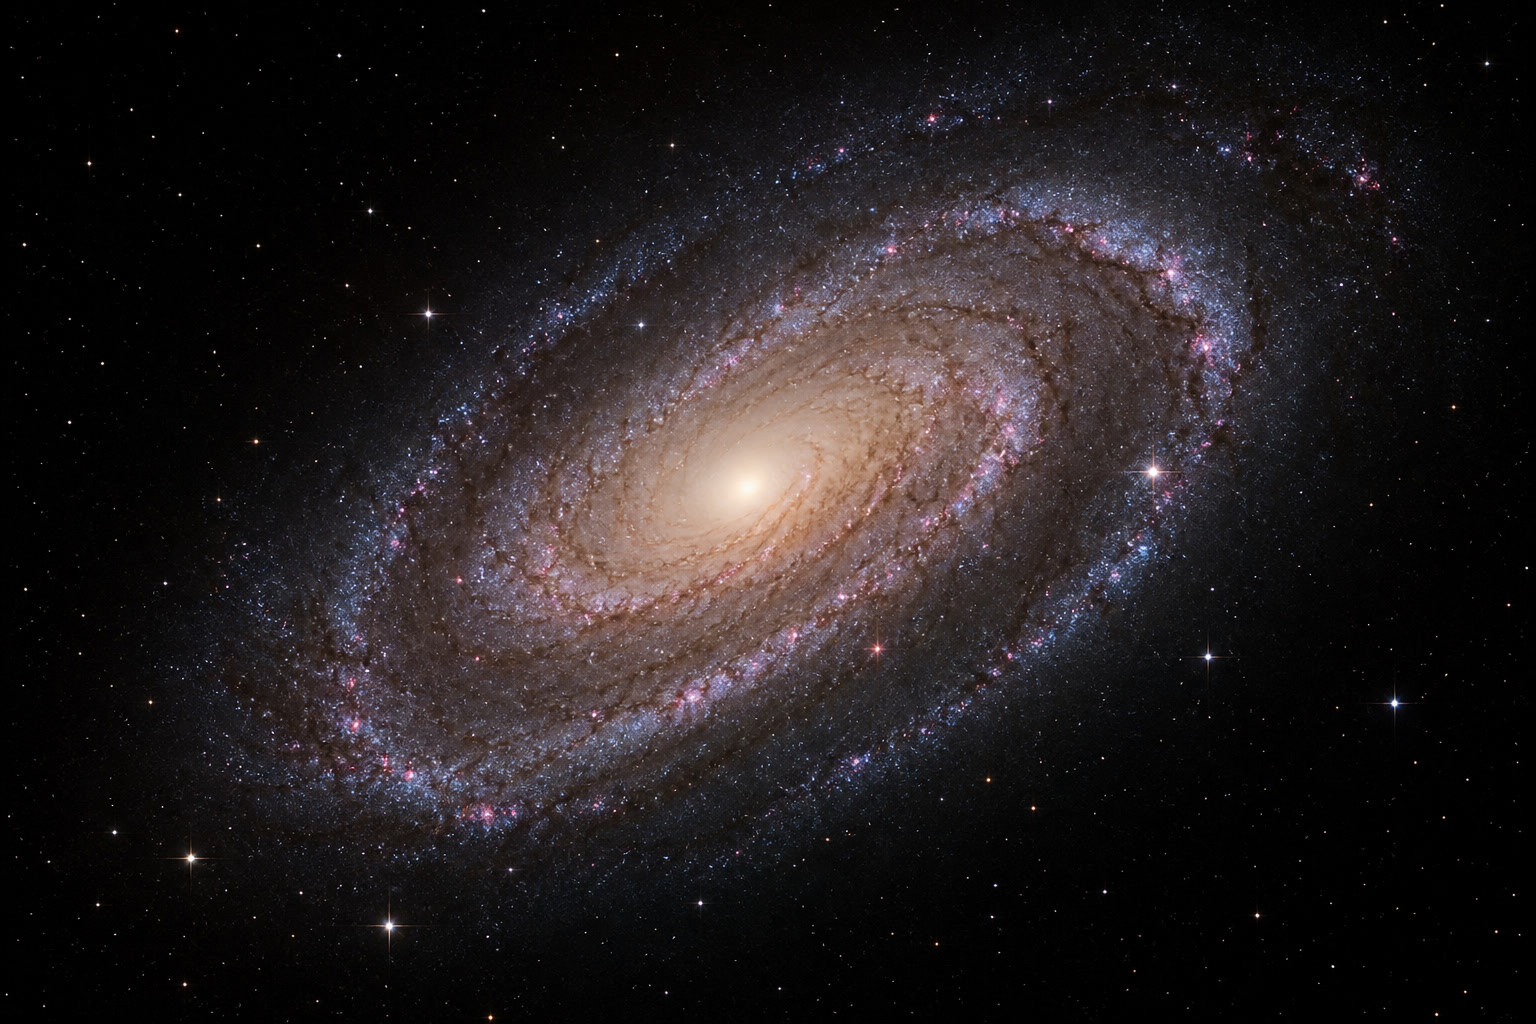
\includegraphics[width=0.55\linewidth]{images/book1/ai/g8-universe-galaxy.jpg}

{\small Une galaxie spirale~: la \omterm{def:g1:light-and-shadows:source}{lumière} de ses \omterm{def:g4:solar-system:star}{étoiles} traverse des millions d'années d'espace vide avant d'atteindre le moindre télescope.}
\end{omfigure}

\section{L'année-lumière}

\begin{definition}[Année-lumière]\label{def:g8:speed-of-light:lightyear}
Une \emph{année-lumière}\index{année-lumière} est une
\emph{distance}~: le chemin que la \omterm{def:g1:light-and-shadows:source}{lumière} parcourt en un an ---
environ $9.5 \times 10^{12}$ km, près de dix millions de millions de
kilomètres. Le nom égare les pressés (ce n'est pas plus une \omterm{def:g2:measuring-time:duration}{durée}
qu'un «~pas~» n'est un pied)~; les astronomes s'en servent parce que
les kilomètres s'effondrent sous la véritable échelle du ciel.
\end{definition}

\begin{example}[Le voisinage en années-lumière]\label{ex:g8:speed-of-light:ladder}
L'\omterm{def:g4:solar-system:star}{étoile} la plus proche après le Soleil~: environ $4$
\omterm{def:g1:light-and-shadows:source}{années-lumière} --- les grains de \omterm{def:g1:light-and-shadows:source}{lumière} de ce soir l'ont quittée
quand tu en étais à tes premiers chapitres de physique. Les \omterm{def:g4:solar-system:star}{étoiles}
brillantes du ciel d'hiver~: des dizaines à des centaines
d'\omterm{def:g1:light-and-shadows:source}{années-lumière}. La \omterm{ex:g5:stars-night-sky:milkyway}{Voie lactée}, notre cité d'\omterm{def:g4:solar-system:star}{étoiles}~: environ
$100000$ \omterm{def:g1:light-and-shadows:source}{années-lumière} de part en part. La grande galaxie voisine la
plus proche~: quelque $2.5$ millions d'\omterm{def:g1:light-and-shadows:source}{années-lumière} --- sa faible
tache, visible à l'œil nu accoutumé à l'obscurité, est la plus
ancienne \omterm{def:g1:light-and-shadows:source}{lumière} qu'un humain puisse voir sans aide.
\end{example}

\begin{proposition}[Les télescopes sont des machines à remonter le temps]\label{prop:g8:speed-of-light:timemachine}
Parce que les nouvelles de la \omterm{def:g1:light-and-shadows:source}{lumière} voyagent à $c$ et que l'Univers
est vaste, \emph{regarder loin, c'est regarder en arrière}. L'\omterm{def:g4:solar-system:star}{étoile} à
$4$ \omterm{def:g1:light-and-shadows:source}{années-lumière} se montre telle qu'elle était il y a $4$ ans~; la
galaxie voisine, telle qu'elle était quand nos ancêtres taillaient
leurs premiers outils de pierre. Le soupçon de l'observateur d'\omterm{def:g4:solar-system:star}{étoiles}
du grade 5 est maintenant un théorème d'arithmétique~: tout télescope
pointé vers le dehors est pointé vers le passé, et l'astronomie est
l'histoire lue à la \omterm{def:g1:light-and-shadows:source}{lumière} des \omterm{def:g4:solar-system:star}{étoiles}.
\end{proposition}

\begin{method}[Convertir distance et regard en arrière]\label{met:g8:speed-of-light:convert}
\begin{enumerate}
  \item distance en \omterm{def:g1:light-and-shadows:source}{années-lumière} $\to$ regard en arrière en
        années~: le même nombre --- tout le génie de cette \omterm{def:g6:measurement-in-science:measuring}{unité} est
        là~;
  \item distance en kilomètres $\to$ temps de \omterm{def:g1:light-and-shadows:source}{lumière}~: diviser par
        \qty{300000}{km/s}, puis dompter les secondes en minutes, en
        \omterm{ex:g2:measuring-time:clock}{heures} ou en années~;
  \item \omterm{def:g1:light-and-shadows:source}{années-lumière} $\to$ kilomètres (rarement utile)~:
        multiplier par $9.5 \times 10^{12}$ --- et se rappeler
        pourquoi les astronomes le font rarement.
\end{enumerate}
\end{method}

\begin{remark}[Ce que «~maintenant~» veut dire là-haut]\label{rem:g8:speed-of-light:now}
L'\omterm{def:g4:solar-system:star}{étoile} à quatre \omterm{def:g1:light-and-shadows:source}{années-lumière} brille-t-elle encore \emph{en ce
moment même}~? Presque sûrement --- les \omterm{def:g4:solar-system:star}{étoiles} vivent longtemps ---
mais aucune réponse plus rapide que la \omterm{def:g1:light-and-shadows:source}{lumière} elle-même ne peut nous
parvenir~: la nouvelle la plus fraîche possible a quatre ans, toujours.
Pour le ciel profond, la question se ramollit en étrangeté~: certaines
des taches les plus faibles des grands télescopes sont des galaxies
dont la \omterm{def:g1:light-and-shadows:source}{lumière} est partie avant l'existence de la Terre. La physique
affinera dans les années d'université ce que «~maintenant, à
distance~» peut seulement vouloir dire~; pour cette année, emporte la
version honnête~: le ciel n'est pas une scène --- c'est une archive.
\end{remark}

\section{Exercices}

\begin{exercise}[$\star$]\label{exo:g8:speed-of-light:1}
Donne $c$ en \unit{km/s} et en \unit{m/s} (en puissances de dix).
Qu'est-ce qui a échoué sur les deux collines, et pourquoi~?
\end{exercise}

\begin{exercise}[$\star$]\label{exo:g8:speed-of-light:2}
Raconte de nouveau l'argument du satellite en retard en trois
phrases~: qu'est-ce qui était ponctuel, qu'est-ce qui était en
retard, et qu'a mesuré ce retard~?
\end{exercise}

\begin{exercise}[$\star$]\label{exo:g8:speed-of-light:3}
Calcule le temps de trajet de la \omterm{def:g1:light-and-shadows:source}{lumière}~: la \omterm{def:g2:moon-in-the-sky:moon}{Lune}
(\qty{384000}{km})~; le Soleil ($150$ millions de km). Pourquoi la
\omterm{def:g1:light-and-shadows:source}{lumière} du Soleil est-elle une «~vieille nouvelle~»~?
\end{exercise}

\begin{exercise}[$\star$]\label{exo:g8:speed-of-light:4}
Une \omterm{def:g8:speed-of-light:lightyear}{année-lumière} --- \omterm{def:g2:measuring-time:duration}{durée} ou distance~? Définis-la, et donne sa
taille en kilomètres (en puissances de dix).
\end{exercise}

\begin{exercise}[$\star$]\label{exo:g8:speed-of-light:5}
L'\omterm{def:g4:solar-system:star}{étoile} la plus proche se tient à environ $4$ \omterm{def:g1:light-and-shadows:source}{années-lumière}. Quel
est le regard en arrière de ce soir --- et que faisais-tu quand sa
\omterm{def:g1:light-and-shadows:source}{lumière} est partie~?
\end{exercise}

\begin{exercise}[$\star$]\label{exo:g8:speed-of-light:6}
Pourquoi personne ne peut-il piloter un rover martien au manche à
balai depuis la Terre~? Sers-toi des nombres de l'exemple de
l'horaire.
\end{exercise}

\begin{exercise}[$\star$]\label{exo:g8:speed-of-light:7}
Classe par profondeur de regard en arrière~: la \omterm{def:g2:moon-in-the-sky:moon}{Lune}~; le Soleil~;
l'\omterm{def:g4:solar-system:star}{étoile} la plus proche~; la galaxie voisine --- avec l'ordre de
grandeur de chacun.
\end{exercise}

\begin{exercise}[$\star$]\label{exo:g8:speed-of-light:8}
«~Le \omterm{def:g2:measuring-length:units}{mètre} se définit désormais à partir de $c$.~» Que dit cela sur
celui des deux --- la règle ou la \omterm{def:g1:light-and-shadows:source}{lumière} --- auquel les physiciens se
fient le plus profondément~?
\end{exercise}

\begin{exercise}[$\star\star$]\label{exo:g8:speed-of-light:9}
Télémétrie radar~: une impulsion radio (voyageant à $c$) renvoyée par
la \omterm{def:g2:moon-in-the-sky:moon}{Lune} revient en environ \qty{2.6}{s}. Retrouve la distance de la
\omterm{def:g2:moon-in-the-sky:moon}{Lune} à partir de cet aller-retour --- et nomme la vieille règle du
sonar qui se transpose ici.
\end{exercise}

\begin{exercise}[$\star\star$]\label{exo:g8:speed-of-light:10}
Classe par profondeur d'archive~: la \omterm{def:g1:light-and-shadows:source}{lumière} d'une lampe dans ta
chambre (\qty{3}{m})~; le Soleil~; une \omterm{def:g4:solar-system:star}{étoile} à $100$
\omterm{def:g1:light-and-shadows:source}{années-lumière}~; la galaxie voisine. Pour la lampe, estime le regard
en arrière en milliardièmes de seconde ($3 \div (3 \times 10^{8})$ ---
dompte-le avec des mots).
\end{exercise}

\begin{exercise}[$\star\star$]\label{exo:g8:speed-of-light:11}
Un bulletin d'information annonce~: «~des astronomes ont vu une \omterm{def:g4:solar-system:star}{étoile}
exploser mardi dernier, à $8000$ \omterm{def:g1:light-and-shadows:source}{années-lumière} d'ici.~» Réécris la
phrase avec des temps honnêtes~: quand l'explosion a-t-elle eu lieu,
et que s'est-il passé mardi dernier~?
\end{exercise}

\begin{exercise}[$\star\star\star$]\label{exo:g8:speed-of-light:12}
Le retard du satellite culmine à environ $1000$ secondes --- le temps
qu'il faut à la \omterm{def:g1:light-and-shadows:source}{lumière} pour franchir toute la largeur de l'\omterm{def:g6:sun-earth-moon:axisorbit}{orbite}
terrestre, environ $3 \times 10^{8}$ km. Fais toi-même la division du
dix-septième siècle et compare au $c$ moderne~: quelle honnêteté
avait la première réponse du ciel~?
\end{exercise}

\section{Problème~: le centre de contrôle}

\begin{problem}[{Problème du week-end --- une garde au centre de
contrôle des missions lointaines~; des conversations retardées par la
lumière, de la Lune aux étoiles~; le manuel
d'exploitation}]\label{pb:g8:speed-of-light:1}
Ce soir, tu diriges le pupitre des communications~: tout message
voyage à $c = \qty{300000}{km/s}$, et le retard de la \omterm{def:g1:light-and-shadows:source}{lumière}
gouverne chaque décision.

\medskip\noindent\textbf{Partie I --- les opérations proches.}
\begin{enumerate}
  \item La base lunaire (\qty{384000}{km}) demande confirmation d'un
        largage de ravitaillement. Combien de temps après ton
        «~confirmé~» la base l'entend-elle, et au plus tôt quand
        peux-tu entendre son accusé de réception~?
  \item Un satellite en \omterm{def:g6:sun-earth-moon:axisorbit}{orbite} haute, à \qty{36000}{km}, relaie un
        signal de télévision. Calcule son retard aller simple --- et
        dis pourquoi les appels téléphoniques intercontinentaux
        passant par de tels satellites portent une hésitation tout
        juste perceptible (aller-retour, montée et descente).
  \item L'observatoire solaire signale une grande éruption
        «~en direct~». Corrige la formule de l'opérateur~: quand
        l'éruption a-t-elle vraiment jailli~?
  \item Le protocole exige que toutes les horloges tiennent compte
        du retard. Quelle liaison proche de la Terre --- la \omterm{def:g2:moon-in-the-sky:moon}{Lune} ou
        le satellite haut --- demande la plus grande marge, et
        approximativement dans quel rapport~?
\end{enumerate}

\medskip\noindent\textbf{Partie II --- la fenêtre martienne.}
Mars se tient ce soir à $1.8 \times 10^{8}$ km.
\begin{enumerate}[resume]
  \item Calcule le retard aller simple en secondes, puis en minutes.
  \item Le rover rencontre une crevasse imprévue et ses caméras le
        montrent qui s'en approche au pas. Explique, avec le chiffre
        de l'aller-retour, pourquoi un sauvetage au manche à balai
        est sans espoir --- et ce que le rover doit donc emporter à
        son bord.
  \item Le téléversement du plan de la soirée demande \qty{3}{min}
        de transmission, plus le retard. À quelle heure faut-il
        commencer le téléversement pour qu'il soit intégralement
        reçu par le rover à 21:00, heure du contrôle~?
  \item Dans six mois, Mars se tiendra à $3.8 \times 10^{8}$ km.
        Que devient le retard, et que nous apprend cela sur «~la~»
        distance à une \omterm{def:g4:solar-system:planet}{planète}~?
\end{enumerate}

\medskip\noindent\textbf{Partie III --- le pupitre du lointain.}
\begin{enumerate}[resume]
  \item Une sonde interstellaire a atteint un plein
        \emph{jour}-lumière de la Terre. Exprime cette distance en
        kilomètres (en puissances de dix~; un jour compte $86400$
        secondes), et donne le temps d'une conversation
        aller-retour avec la sonde.
  \item Les rêveurs du pupitre du fond rédigent un «~message à
        l'\omterm{def:g4:solar-system:star}{étoile} la plus proche~». Rédige plutôt le calendrier~:
        envoyé ce soir, au plus tôt quand une réponse
        arriverait-elle~?
  \item Le mur des archives montre l'\omterm{prop:g5:mirrors-reflection:image}{image} profonde de ce soir de la
        galaxie voisine, à $2.5$ millions d'\omterm{def:g1:light-and-shadows:source}{années-lumière}. Ajoute
        au cartel le temps honnête qui convient --- quelle époque du
        passé de la Terre cet instantané rediffuse-t-il là-bas, si
        quelqu'un s'y trouvait pour regarder~?
  \item Journal de fin de garde~: écris les trois règles du
        pupitre --- une sur l'instantané (à savoir que rien ne
        l'est), une sur les manches à balai et le retard, une sur
        les télescopes et l'archive.
\end{enumerate}
\end{problem}
